%%%%%%%%%%%%%%%%%%%%%%%%%%% asme2e.tex %%%%%%%%%%%%%%%%%%%%%%%%%%%%%%%
% Template for producing ASME-format articles using LaTeX            %
% Written by   Harry H. Cheng                                        %
%              Integration Engineering Laboratory                    %
%              Department of Mechanical and Aeronautical Engineering %
%              University of California                              %
%              Davis, CA 95616                                       %
%              Tel: (530) 752-5020 (office)                          %
%                   (530) 752-1028 (lab)                             %
%              Fax: (530) 752-4158                                   %
%              Email: hhcheng@ucdavis.edu                            %
%              WWW:   http://iel.ucdavis.edu/people/cheng.html       %
%              May 7, 1994                                           %
% Modified: February 16, 2001 by Harry H. Cheng                      %
% Modified: January  01, 2003 by Geoffrey R. Shiflett                %
% Use at your own risk, send complaints to /dev/null                 %
%%%%%%%%%%%%%%%%%%%%%%%%%%%%%%%%%%%%%%%%%%%%%%%%%%%%%%%%%%%%%%%%%%%%%%

%%% use twocolumn and 10pt options with the asme2e format
\documentclass[twocolumn,10pt]{asme2e}
\special{papersize=8.5in,11in}
\usepackage{graphicx}
\graphicspath{{./}}
\usepackage[%  
    colorlinks=true,
    pdfborder={0 0 0},
    linkcolor=red
]{hyperref}

%% The class has several options
%  onecolumn/twocolumn - format for one or two columns per page
%  10pt/11pt/12pt - use 10, 11, or 12 point font
%  oneside/twoside - format for oneside/twosided printing
%  final/draft - format for final/draft copy
%  cleanfoot - take out copyright info in footer leave page number
%  cleanhead - take out the conference banner on the title page
%  titlepage/notitlepage - put in titlepage or leave out titlepage
%  
%% The default is oneside, onecolumn, 10pt, final

%%% Replace here with information related to your conference
%\confshortname{IDETC/CIE 2009}
%\conffullname{the ASME 2009 International Design Engineering Technical Conferences \&\\
    %          Computers and Information in Engineering Conference}

%%%%% for date in a single month, use
%\confdate{24-28}
%\confmonth{September}
%%%%% for date across two months, use
%\confdate{January 6-September 2}
%\confyear{2009}
%\confcity{San Diego}
%\confcountry{USA}

%%% Replace DETC2009/MESA-12345 with the number supplied to you 
%%% by ASME for your paper.
%\papernum{DETC2009/MESA-12345}

%%% You need to remove 'DRAFT: ' in the title for the final submitted version.
\title{Overcoming the memory bound of Big Data Analytics to improve server throughput using fast storage} 
%%% for the discussion section only
%\usepackage{helvet}
%\title{\fontfamily{phv}\selectfont{\Huge{DRAFT: AN ARTICLE CREATED USING \LaTeX2\raisebox{-.3ex}{$\epsilon$}\ IN ASME FORMAT}}}

%%% first author
\author{Emmanouil Anagnostakis
    \affiliation{
	    Graduate Research Assistant\\
	    Computer Architecture and VLSI Systems Laboratory, ICS-FORTH\\
	    Heraklion, Greece\\
      manosanag@ics.forth.gr
    }	
}

%%% second author
%%% remove the following entry for single author papers
%%% add more entries for additional authors
%\author{First Coauthor\thanks{Address all correspondence to this author.} \\
%       {\tensfb Second Coauthor}     
%    \affiliation{Department or Division Name\\
%	Company or College Name\\
%	City, State (spelled out), Zip Code\\
%	Country (only if not U.S.)\\
%	Email address (if available)
%    }
%}

\begin{document}

\maketitle    

%%%%%%%%%%%%%%%%%%%%%%%%%%%%%%%%%%%%%%%%%%%%%%%%%%%%%%%%%%%%%%%%%%%%%%
\section*{Abstract}

Managing big data analytics i.e. Apache Spark poses challenges due to limited memory resources in data centers. The memory pressure that arises during data processing can result in low server throughput, causing delays and inefficiencies. Memory is wasted in long GC (Garbage Collection) cycles leaving no room for useful work. In this paper, we propose a novel approach to improve server throughput for managed big data analytics using smart heap offloading to fast storage devices and reducing memory pressure. Our approach involves offloading data from heap memory to fast storage devices in a smart and efficient manner, thereby freeing up heap memory and reducing memory pressure without suffering from storage latencies. By overcoming the memory bound we leave space to the applications for more CPU utilization. We present a detailed methodology for running Apache Spark using our proposed mechanism of smart heap offloading, which significantly improves server throughput for managed big data analytics. We implement our proposed approach in Oracle's OpenJDK8 and evaluate its performance using various workloads of the Spark Bench suite on a real-world cluster. Our experimental results show that our approach significantly improves server throughput while reducing memory usage against native Spark, making it a promising solution for managed big data analytics in data centers. We also include results to show that our implementation can reduce money cost if deployed in a world cluster like Amazon's EC2 or Google Cloud Platform or Microsoft Azure Cloud which are available to everyone. 

%%%%%%%%%%%%%%%%%%%%%%%%%%%%%%%%%%%%%%%%%%%%%%%%%%%%%%%%%%%%%%%%%%%%%%
\section*{1. Introduction}

With the exponential growth of data in various fields such as finance, healthcare, social media, and e-commerce, there is a significant need for scalable and efficient big data processing frameworks. Apache Spark \cite{Spark} is one such framework that has gained popularity due to its ability to handle large-scale data processing and analytics. Spark provides a distributed computing platform that can process data in parallel across multiple nodes in a cluster. However, with the increasing size and complexity of big data workloads, Spark clusters are facing significant challenges in meeting the performance and throughput requirements.

One of the main challenges in Spark clusters is the high computational and memory requirements of big data analytics workloads. These requirements can result in excessive CPU and memory usage on Spark workers, leading to performance bottlenecks and slow job completion times. To address these challenges, researchers have proposed various techniques to optimize the performance of Spark clusters, including data partitioning, caching, and resource allocation.

In this paper, we focus on the memory limit problem of servers becoming an obstacle for further throughput increase and we propose a new technique for improving the performance and job throughput of Spark clusters by moving long-lived objects from the main managed Java Heap to a fast storage device such as NVMe, thereby saving memory for other more useful tasks and leaving space for more CPU utilization. Our approach leverages the capabilities of the underlying machine to create less memory-consuming computation tasks, thereby reducing the workload on the Spark workers to improve job throughput, while maintaining effective single instance performance under the colocation of multiple instances required to achieve max throughput.

Specifically, in order to achieve higher throughput and better performance for Spark, we use TeraHeap, a secondary managed memory-mapped heap over an NVMe storage device, which is used to hold the Resilient Distributed Datasets (Spark RDDs) instead of the main managed Java Heap and completely remove any Serialization/Deserialization and Garbage Collection (GC) cost over them.

TeraHeap 1) eliminates Serialization/Deserialization overheads posed by this kind of frameworks when moving data off-heap to/from fast storage devices 2) eliminates GC pauses over the secondary heap, therefore significantly minimizing overall GC overhead. By offloading the managed Java Heap and relaxing computation-intensive tasks, we aim to reduce the workload on Spark workers, thereby improving their performance and job throughput. We also explore the trade-offs between the cost of offloading and the performance gains achieved.

We demonstrate the effectiveness of our approach using various big data analytics workloads on a real-world Spark cluster. We also compare our approach with the native Spark distribution and show that our approach can be used instead of this distribution to improve performance and server throughput.

The paper makes the following contributions 1) A comprehensive evaluation of the performance and cost trade-offs of creating light-weight computation tasks in Spark clusters. 2) A detailed methodology for running Apache Spark and understanding how to use it for conducting off-heap experiments 3) Proves that heap offloading to fast storage devices is a significant research direction. 

The rest of the paper is organized as follows. In section 2 we discuss related work on Spark optimization techniques and offloading techniques. In section 3, we describe our experimental methodology in order for someone to achieve the desired performance using TeraHeap. In section 4, we present our experimental results and evaluate the performance and cost trade-offs of our approach. In section 5, we discuss future research directions. Finally we conclude the paper in section 6 with an outline of our work.

%%%%%%%%%%%%%%%%%%%%%%%%%%%%%%%%%%%%%%%%%%%%%%%%%%%%%%%%%%%%%%%%%%%%%%
\section*{2. Related Work}

Several studies have been conducted to improve the performance of big data processing systems. One approach is to utilize memory-aware task co-location to improve Spark application throughput, which has been investigated by Marco et al. in [3]. Meanwhile, in [4], Kirisame et al. proposed optimal heap limits to reduce browser memory use. Another research direction is to leverage far memory to improve job throughput, as studied by Amaro et al. in [5]. To facilitate memory offloading in datacenters, Weiner et al. presented TMO, a transparent memory offloading system in [6]. In cloud computing platforms, Sharma et al. proposed per-VM page cache partitioning to improve performance in [7]. Chen and Wang introduced Spark on Entropy, a reliable and efficient scheduler for low-latency parallel jobs in heterogeneous clouds, in [8]. Thamsen et al. developed Mary, Hugo, and Hugo*, three learning-based schedulers for distributed data-parallel processing jobs on shared clusters in [9]. Additionally, Bhimani et al. proposed a lightweight virtualization framework for accelerating big data applications on enterprise cloud in [10], while Zhang et al. focused on understanding and improving disk-based intermediate data caching in Spark in [11]. Finally, Intasorn et al. investigated using compression tables to improve HiveQL performance with Spark in a case study on NVMe storage devices in [12]. 

These studies demonstrate a variety of approaches for optimizing big data processing systems, ranging from memory-aware task co-location and memory offloading to scheduler design and virtualization frameworks. The findings from these studies can provide insights and guidance for future research in the field of big data processing.

%%%%%%%%%%%%%%%%%%%%%%%%%%%%%%%%%%%%%%%%%%%%%%%%%%%%%%%%%%%%%%%%%%%%%%
\section*{3. Experimental Methodology}

To evaluate the effectiveness of our proposed approach, we conduct a set of experiments using various workloads from the Spark Bench suite on a real-world cluster. Our experimental methodology consists of several steps. First, we set up our research server, using various configurations of datacenter machines, including CPU, memory, and storage. Next, we install and configure Spark and OpenJDK8 on the cluster. We use Spark's default configuration settings for our experiments, except for the garbage collector settings, which we tune according to our proposed approach.

We select two workloads from the Spark Bench suite that represent different types of data processing, such as machine learning and graph processing, (and SQL queries ???). We run each workload using our proposed approach and compare it with the performance of the same workload using the default configuration, garbage collector tuning, and heap offloading approaches.

We use all the DRAM provided by our server leaving 8-10 GB for Operating System, while increasing the number of Spark instances that are executed. We show that by using TeraHeap, each individual instance requires less memory therefore memory becomes available for more instances to be deployed, achieving more total throughput than Native Spark in similar time windows.

To measure the performance of our approach, we use several metrics, including server throughput, memory usage, and execution time. We measure server throughput as the megabytes of the dataset processed per second, memory usage as the amount of memory used during data processing, and execution time as the time taken to complete the workload.

We repeat each experiment several times to ensure statistical significance and calculate the mean and standard deviation of the metrics for each approach.

In summary, our experimental methodology involves setting up a real-world cluster, selecting appropriate workloads, measuring performance using several metrics, and repeating each experiment several times to ensure statistical significance. By following this methodology, we can evaluate the effectiveness of our proposed approach for improving server throughput for managed big data analytics.

\subsection*{3.1 Server Characteristics}
The server used in our experiments is a high-performance machine with hardware specifications found in real-world clusters like Amazon EC2. It is equipped with 8x DDR4 32-GB 2.4 GHz 64-bit DIMMs, providing a total of 256 GB of memory. The DDR4 memory technology is known for its high bandwidth and low power consumption, making it ideal for data-intensive applications like big data analytics. The server also features 32x Intel Xeon E5-2630 2.4 GHz 64-bit CPUs, spanning 2 NUMA islands, each with 512 KB L1, 2 MB L2, and 20 MB L3 (LLC) cache. The Xeon E5-2630 CPU is a high-performance processor designed for data centers, offering a high core count, high clock speed, and advanced features like hyper-threading and Turbo Boost. The large L3 cache helps reduce memory latency, enabling faster data access for CPU-bound workloads. In addition to the powerful CPUs and memory, the server also has 2x KVS NVMe storage devices. NVMe is a high-performance storage technology that uses PCIe to connect directly to the CPU, providing low latency and high throughput. The KVS (Key-Value Store) storage devices are designed for fast, random access to data, making them ideal for storing and retrieving large amounts of data in big data applications. Overall, the server's hardware specifications make it a powerful platform for conducting experiments on managed big data analytics and evaluating the performance of our proposed approach. 

\subsection*{3.2 Native Spark Configuration}
We use Spark v3.3.0 with Kryo Serializer, a state-of-the-art highly optimized S/D Library for Java that Spark recommends. We run Spark with Native OpenJDK8 as a baseline. We use the Parallel Scavenge garbage collector which is the one TeraHeap is implemented for. Parallel Scavenge is also the go-to collector for applications that need high throughput like Spark. We use an executor with eight mutator threads for each instance of Spark we deploy on our server. For Parallel Scavenge, we use 8 GC Threads for minor GC and the default single-threaded old generation GC. Table XXX summarizes the Spark configuration we use as baseline. Spark uses the MEMORY-AND-DISK storage level to place executor memory (heap) in DRAM and cache RDDs in the on-heap cache, up to 50\% of the total heap size. Any remaining RDDs are serialized in the off-heap cache over an NVMe SSD. This device is also used by Spark for shuffling. We run each instance of Spark in a cgroup containing two JVM instances, one for Spark driver and one for Spark executor and all the processes needed to measure performance for this instance. Each cgroup has a limited DRAM Budget. A part of the budget is the capacity of the Java Heap which, for the rest of the paper, we call H1. We do this in order to be sure that every instance of Spark running on our server has a fair amount of DRAM available for it to use. We choose to try two different amounts for H1, 40\% and 80\% of total DRAM budget. 80\% is the go-to percentage of total DRAM RedHat uses in its datacenters [?]. What remains is used by JVM for Native memory (i.e. CodeCache) and for the operating system's Page Cache. In order to avoid inter-NUMA island interference we shut down the 16 cores belonging to the second island thus leaving 16 active cores. We also turn off the swapper, because it adds significant overhead and clouds our ability to better understand the results of the experiments conducted.

\subsection*{3.3 TeraHeap}
\subsubsection*{3.3.1 What is TeraHeap?}
TeraHeap is a high-capacity managed heap that is memory-mapped over a fast storage device (preferrably block-addresable NVMe or byte-addresable NVM). The high speeds these kind of devices operate in, erase any overhead caused by the use of MMIO. TeraHeap is designed as an extension of the main Java Heap. It holds specific long-lived objects that have the same lifetime span. This enables TeraHeap to operate as a GC-free heap that can delete entire regions of objects at once without a need to scan the heap over and over again for dead objects, which would be a performance kill as it would require scans over the storage device. The two main contributions of TeraHeap are the following: 1) MMIO keeps the objects that reside in the storage device deserialized, thus eliminating the need for Serialization/Deserialization, which is the no 1 overhead when running MEMORY-AND-DISK Spark 2) As discussed, TeraHeap reduces GC overheads without wasting DRAM by avoiding scans on long-lived objects, specificaly Spark RDDs.
\subsubsection*{3.3.2 Spark Configuration}
The configuration for TeraHeap is pretty much the same as for Native Spark, with some necessary differences to achieve our goal. TeraHeap is mapped to a different storage device (NVMe) than that Spark is using for shuffling. We do this in order for TeraHeap to utilize its device to its fullest. MMIO allows TeraHeap Spark to run in MEMORY-ONLY storage level as Spark is unaware of using any device and the OS takes control of the I/O. We also make the same decisions for the DRAM budget trying different amounts for H1, 40\% and 80\% of total DRAM budget. By doing that, we have different configurations where H1 dominates PageCache and the reverse showing what the needs of Spark applications are. 

\subsection*{3.4 What workloads did we choose to use for our experiments and why?}
For our experiments, we selected two specific workloads from the Spark Bench suite: PageRank and LinearRegression. The primary reason for selecting these workloads is that they represent different types of big data analytics tasks: PageRank is a graph-based workload, while LinearRegression is a machine learning workload. By selecting workloads from both categories, we can investigate the performance of our proposed approach across a range of big data analytics tasks. Furthermore, both PageRank and LinearRegression are well-established workloads that are commonly used for benchmarking big data analytics systems, making them a suitable choice for our experiments. Overall, the selection of these workloads allows us to evaluate the performance of our approach in a variety of contexts and provide insights into the effectiveness of our approach for improving server throughput in managed big data analytics systems.

\subsubsection*{3.4.1 PageRank}
PageRank is a widely used graph-based algorithm that measures the importance of nodes in a network. It has become a popular benchmark for evaluating the performance of distributed systems, including big data analytics systems like Apache Spark. PageRank is computationally intensive and requires significant memory and I/O resources, making it a suitable workload for evaluating the performance of our proposed approach for improving server throughput. Additionally, PageRank is a common algorithm in real-world applications, such as search engines and social networks, making it relevant for practical use cases.

\subsubsection*{3.4.2 LinearRegression}
LinearRegression is a machine learning algorithm that is used to predict numerical values based on input data. It is a well-known and widely used algorithm in machine learning, and is commonly used for regression analysis in fields such as economics, finance, and engineering. LinearRegression is computationally intensive and requires significant memory and I/O resources, making it a suitable workload for evaluating the performance of our proposed approach for improving server throughput. Furthermore, the inclusion of a machine learning workload like LinearRegression allows us to investigate the performance of our approach across different types of big data analytics tasks and gain insights into the effectiveness of our approach for improving server throughput in a range of contexts.

\begin{figure*}[h!]
        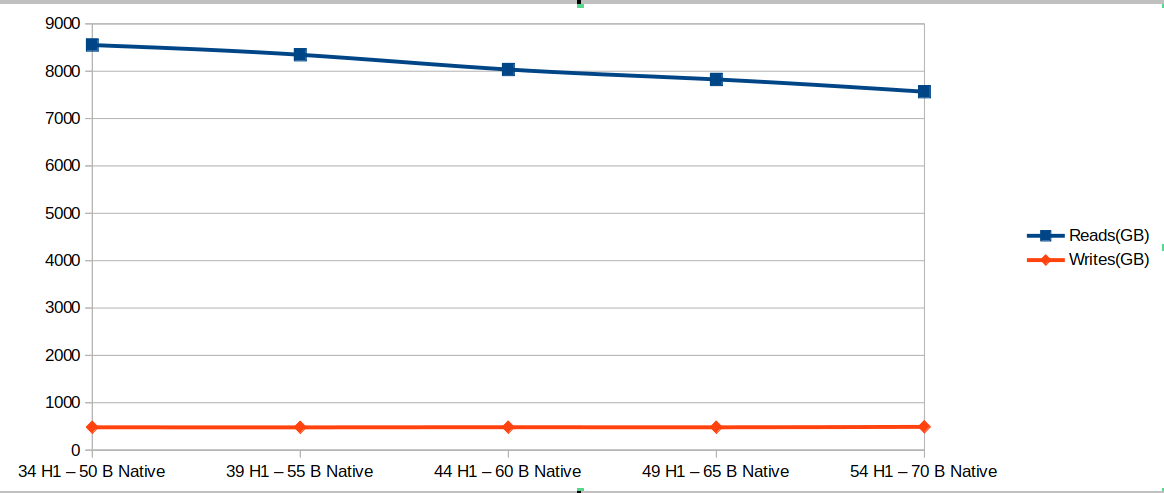
\includegraphics[width=12cm,height=6cm]{gcs_linr_h1_native.png}
\end{figure*}

\begin{figure*}[h!]
        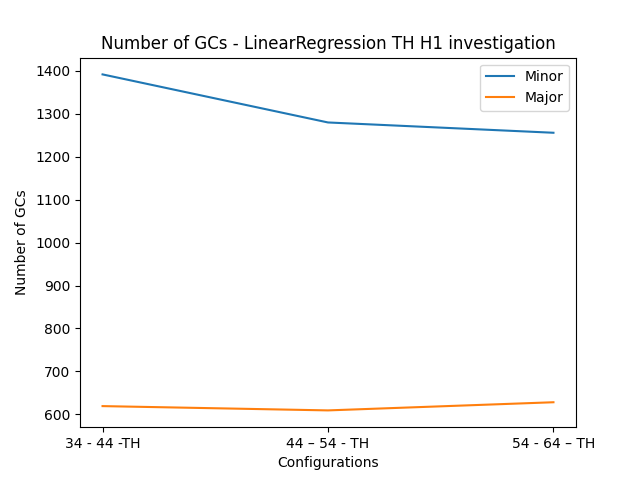
\includegraphics[width=12cm,height=6cm]{gcs_linr_h1_th.png}
\end{figure*}

\begin{figure*}[h!]
        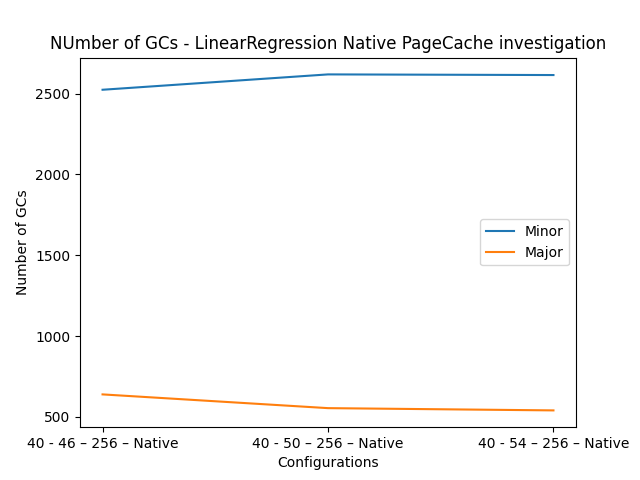
\includegraphics[width=12cm,height=6cm]{gcs_linr_pc_native.png}
\end{figure*}

\begin{figure*}[h!]
        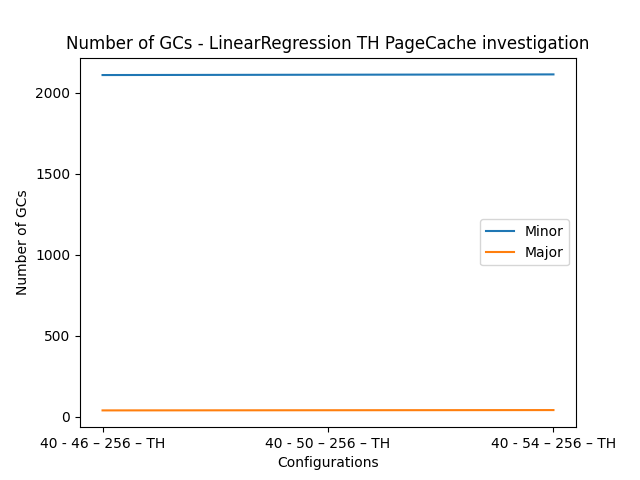
\includegraphics[width=12cm,height=6cm]{gcs_linr_pc_th.png}
\end{figure*}

\begin{figure*}[h!]
        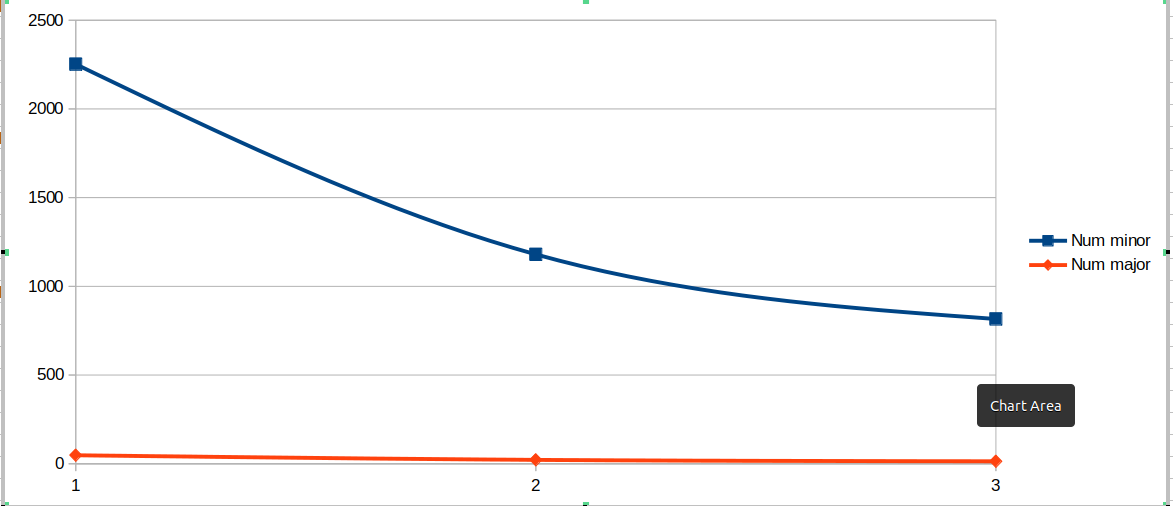
\includegraphics[width=12cm,height=6cm]{gcs_pr_h1_th.png}
\end{figure*}

\begin{figure*}[h!]
        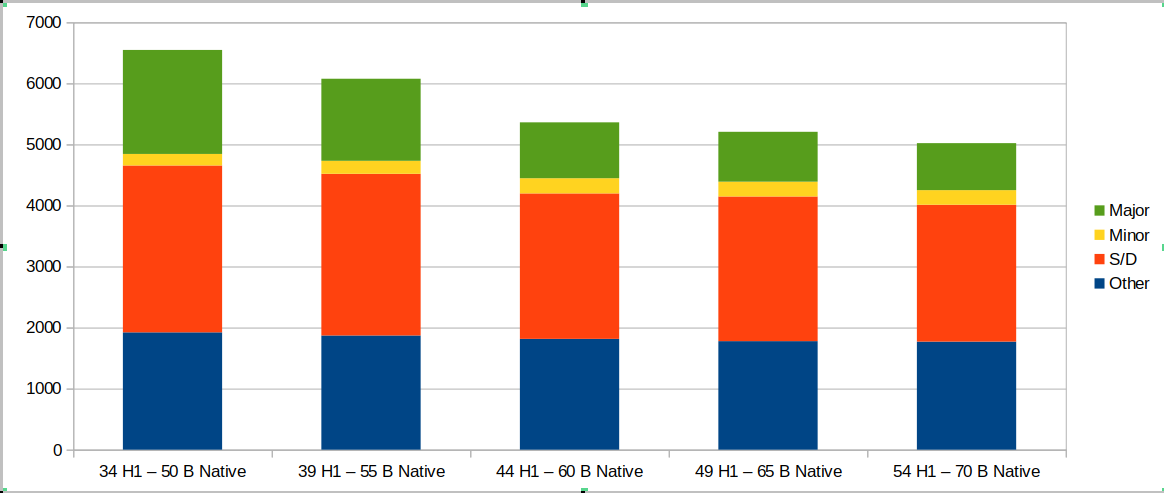
\includegraphics[width=12cm,height=6cm]{linr_h1_native.png}
\end{figure*}

\begin{figure*}[h!]
        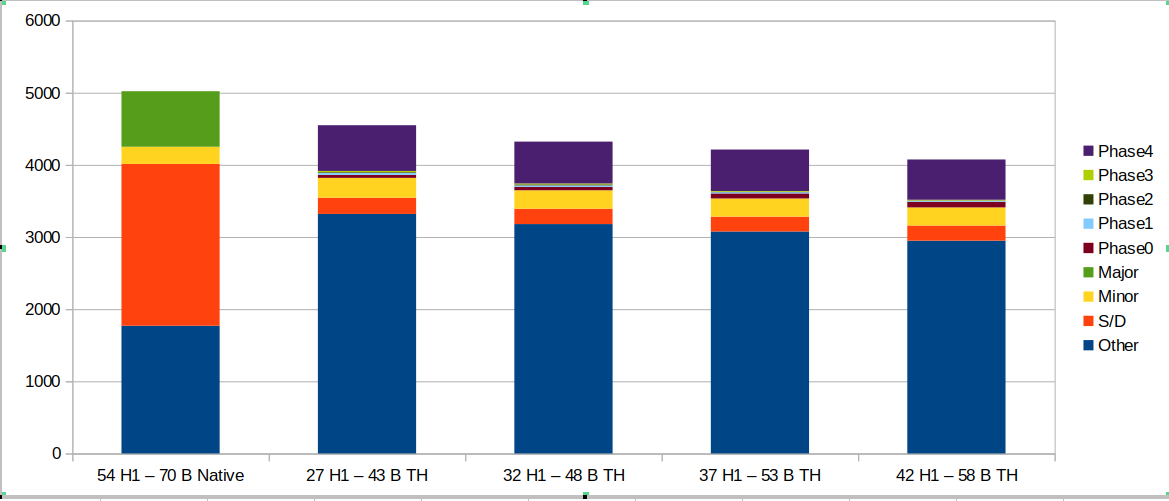
\includegraphics[width=12cm,height=6cm]{linr_h1_th.png}
\end{figure*}

\begin{figure*}[h!]
        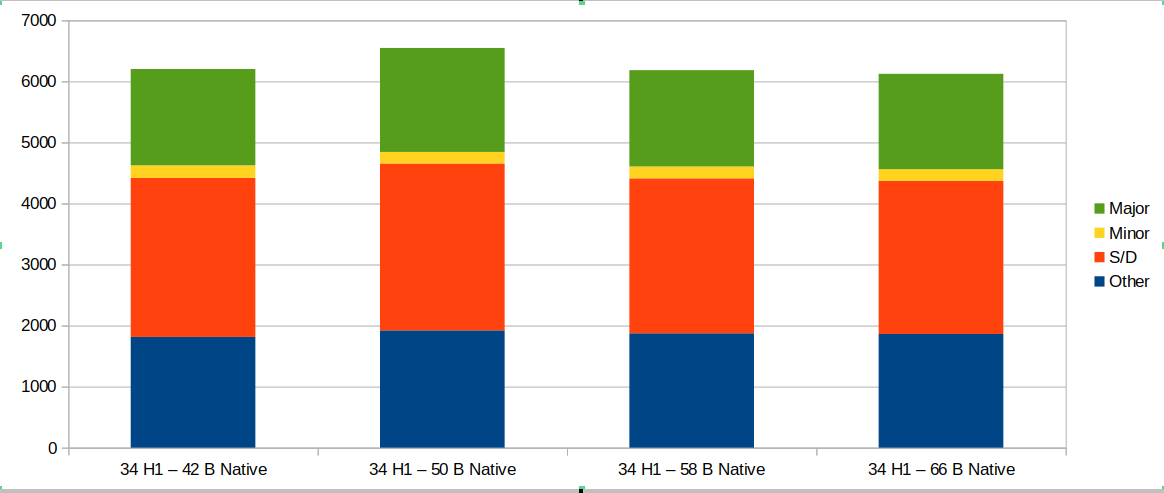
\includegraphics[width=12cm,height=6cm]{linr_pc_native.png}
\end{figure*}

\begin{figure*}[h!]
        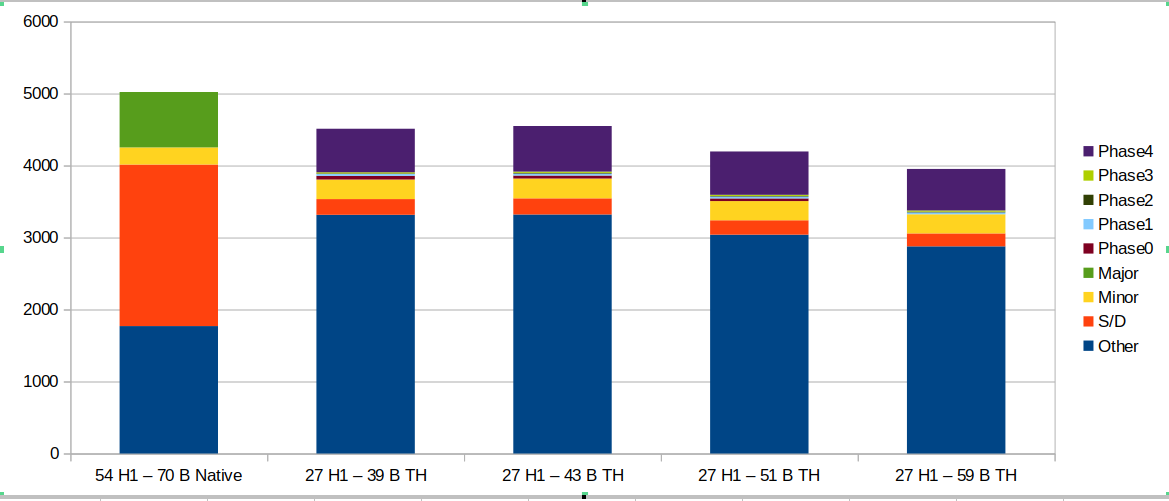
\includegraphics[width=12cm,height=6cm]{linr_pc_th.png}
\end{figure*}

\begin{figure*}[h!]
        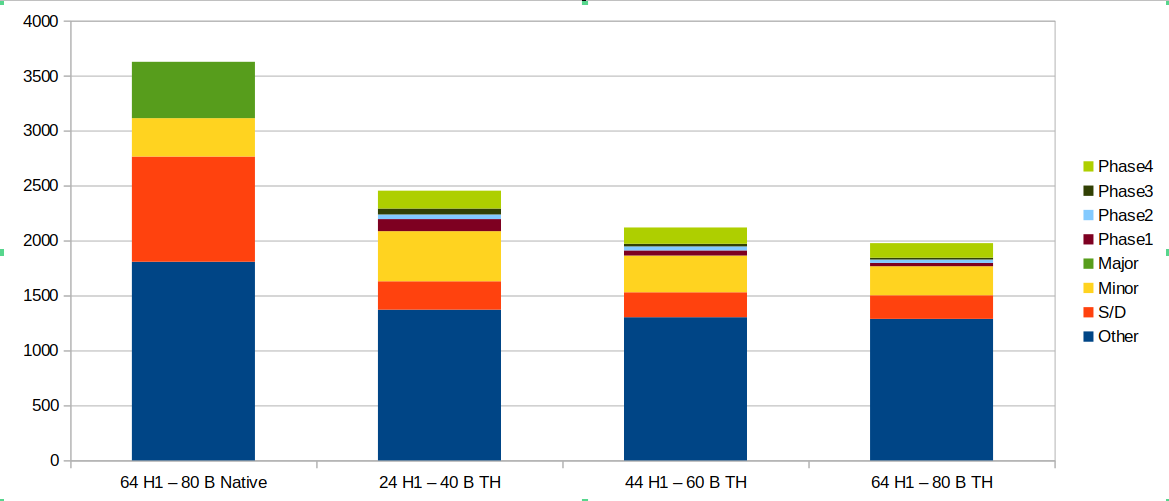
\includegraphics[width=12cm,height=6cm]{pr_h1_th.png}
\end{figure*}

\begin{figure*}[h!]
        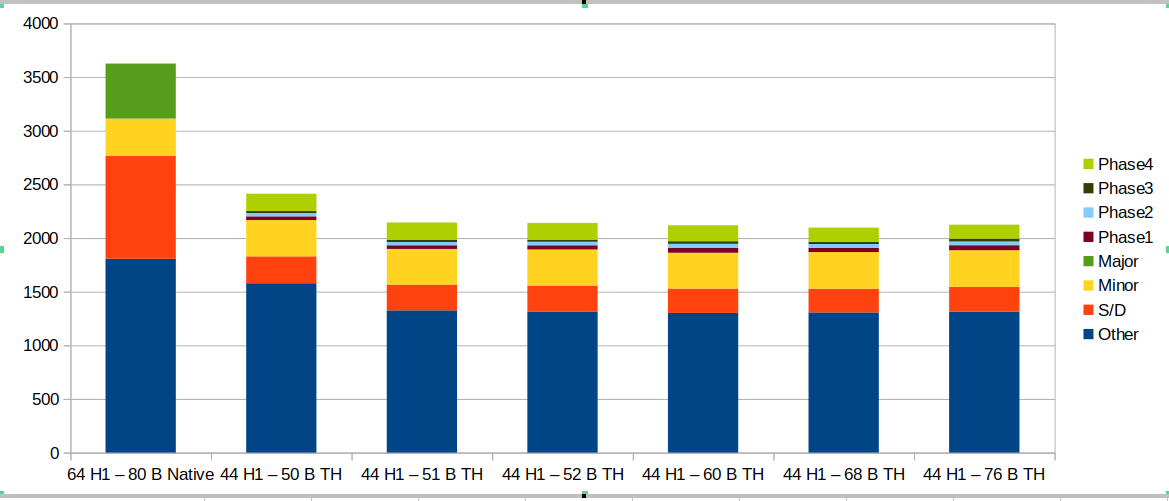
\includegraphics[width=12cm,height=6cm]{pr_pc_th.png}
\end{figure*}

\begin{figure*}[h!]
        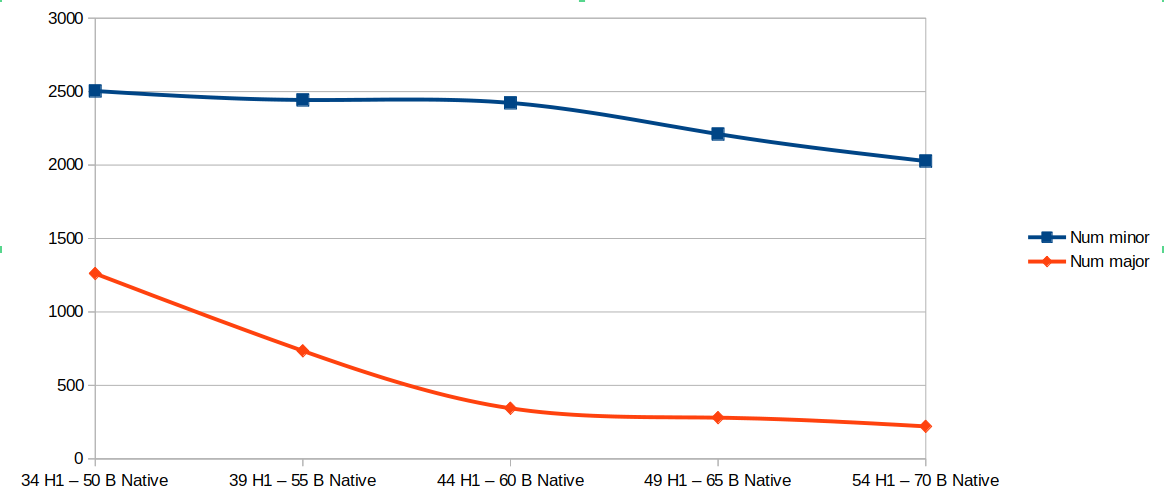
\includegraphics[width=12cm,height=6cm]{rw_linr_h1_native.png}
\end{figure*}

\begin{figure*}[h!]
        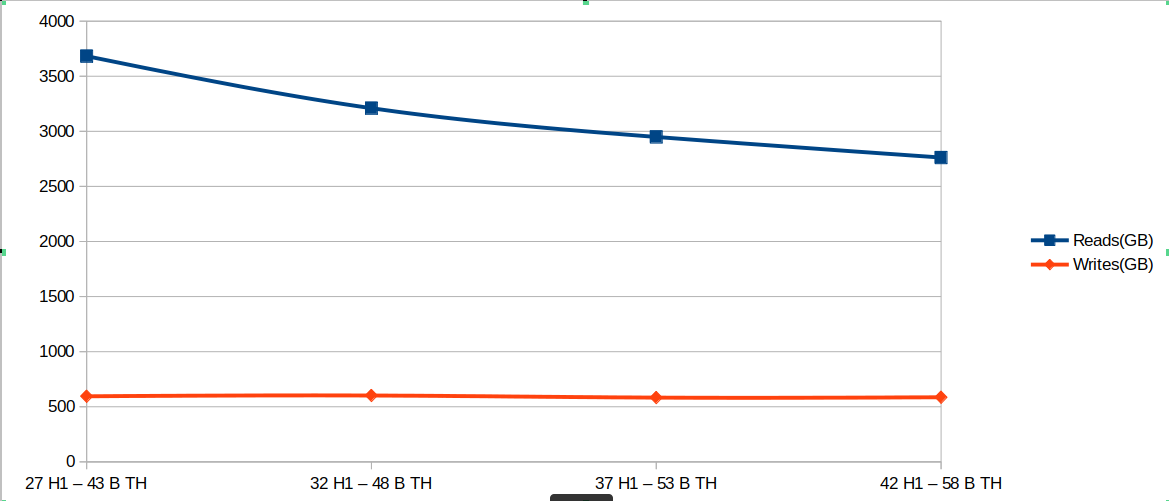
\includegraphics[width=12cm,height=6cm]{rw_linr_h1_th.png}
\end{figure*}

\begin{figure*}[h!]
        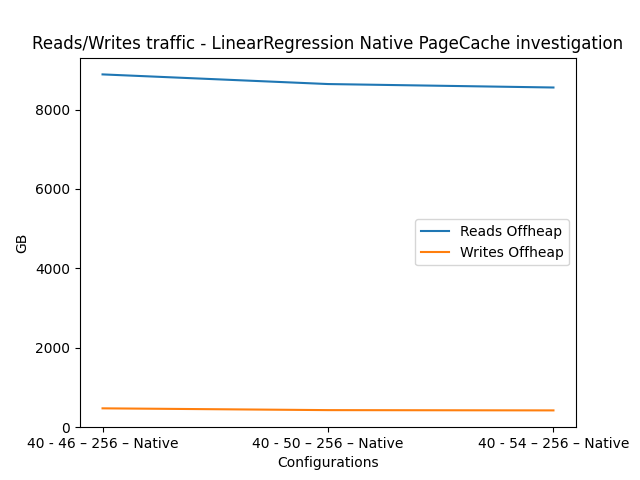
\includegraphics[width=12cm,height=6cm]{rw_linr_pc_native.png}
\end{figure*}

\begin{figure*}[h!]
        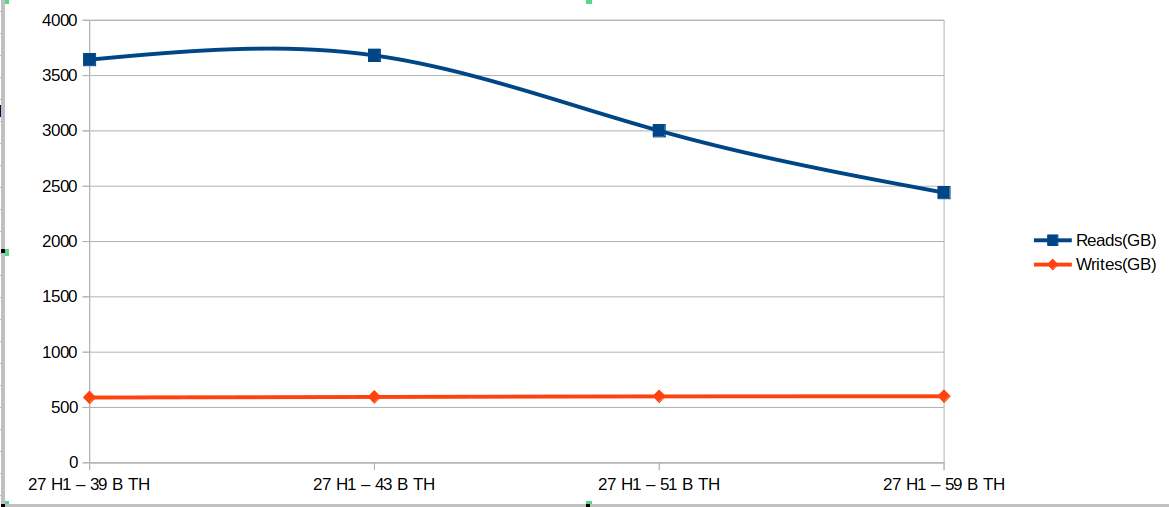
\includegraphics[width=12cm,height=6cm]{rw_linr_pc_th.png}
\end{figure*}

\begin{figure*}[h!]
        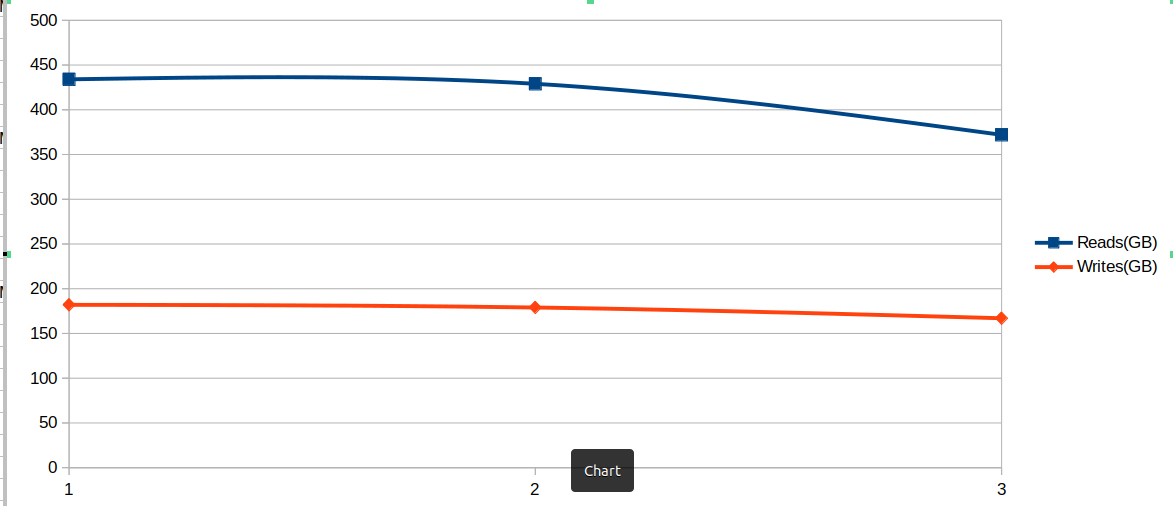
\includegraphics[width=12cm,height=6cm]{rw_pr_h1_th.png}
\end{figure*}

\begin{figure*}[h!]
        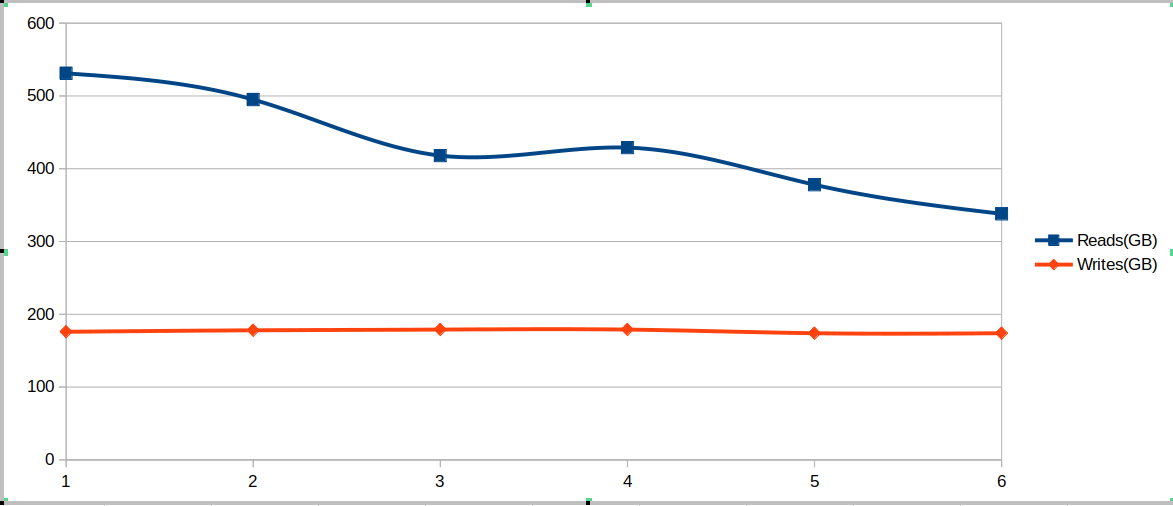
\includegraphics[width=12cm,height=6cm]{rw_pr_pc_th.png}
\end{figure*}

\subsection*{3.5 Is Spark in need of Java Heap or more cache for I/O?}
Still an incomplete prototype subsection.

Spark's memory management is critical for the performance of big data analytics applications. In Spark, memory is divided into three regions: heap memory, execution memory, and storage memory. The heap memory is used for JVM objects and the Spark driver. Execution memory is used for storing data during shuffle and join operations and for caching frequently accessed data. Storage memory is used for storing data that is too large to fit in the execution memory. Spark's memory management system automatically manages the memory allocation and deallocation process based on the workload and available resources. This dynamic allocation helps to avoid memory fragmentation and optimize resource utilization. Additionally, Spark uses a combination of in-memory and disk-based storage to provide efficient data access. Spark provides various storage levels, including MEMORY-ONLY, MEMORY-AND-DISK, and DISK-ONLY, to allow users to balance between memory usage and data availability. We choose MEMORY-AND-DISK to cache 50\% of the RDDs in memory and 50\%s off-heap, in the storage device, to balance memory and storage usage. Spark needs significant amounts of memory even with the use of an off-heap compute cache.
Using off-heap mechanisms denotes I/O and I/O is in need of an I/O cache i.e. the Linux PageCache. Since our spark applications run within a memory-limited cgroup in order to assure fair performance in-between instances, that means that we have to investigate how the different Spark workloads that we are going to use for our evaluation are going to perform with different amounts of H1 (Java Heap) and I/O cache. Increasing/decreasing H1 automaticaly does the opposite to the I/O cache so the mechanism is simple: we manually tune these parameters and investigate how the workloads perform. At first we investigate the performance of TeraHeap Spark regarding these two parameters. Our machine uses 256 GB total DRAM and 16 single-NUMA island CPUs. Figure 1 shows performance of single-instance TeraHeap Spark running PageRank with adjustable size for H1 while PageCache is kept steady at 16 GB. This graph shows that decreasing the size of H1 indicates a significant increase to Minor GC and a slight increase to Major GC. Figure 2 justifies these claims by showing the obvious decrease of the number of minor gcs. Figure 3 shows performance of single-instance TeraHeap Spark running PageRank with adjustable size for PageCache while H1 is kept steady at 44 GB. This graph shows that decreasing the size of PageCache indicates no changes to other time. Figure 4 justifies these claims by showing the obvious decrease of the number of minor gcs. Figure 5... Figure 6 shows performance of single-instance Native Spark running LinearRegression with adjustable size for H1 while PageCache is kept steady at 16 GB. This graph shows that decreasing the size of H1 indicates a significant increase to Major GC and a slight increase to S/D. Other time remains the same. Figure 7 and 8 justify these numbers by showing the number of minor-major gcs to decrease while H1 increases (gc time) and the read-write traffic to remain steady (other). Figure 9 shows performance of single-instance TeraHeap Spark running LinearRegression with adjustable size for PageCache while H1 is kept steady at 27 GB. This graph shows that decreasing the size of PageCache indicates significant changes to Other time. GC time should remain the same as H1 remains steady. Figure 10 and 11 justify these numbers by showing the number of minor-major gcs to remain the same while read traffic decreases as PageCache increases. Figure 12 shows performance of single-instance Native Spark running LinearRegression with adjustable size for H1 while PageCache is kept steady at 16 GB. This graph shows that decreasing the size of H1 indicates a significant increase to Major GC and a slight increase to S/D. Other time remains the same. Figure 13 and 14 justify these numbers by showing the number of minor-major gcs to decrease while H1 increases (gc time) and the read-write traffic to remain steady (other). Figure 15 shows performance of single-instance Native Spark running LinearRegression with adjustable size for PageCache while H1 is kept steady at 34 GB. This graph shows that decreasing the size of PageCache indicates no changes to Other time. So changes to PageCache do not affect this workload. Figure 16 and 17 justify these numbers by showing the number of minor-major gcs as well as read-write traffic to remain the same.
\subsection*{3.6 What kind of metrics should someone use to be accurate when measuring performance?}
When measuring performance, it's important to choose metrics that provide a comprehensive view of the system's behavior. In the case of measuring the performance of Spark instances, there are several key metrics that one should consider. These include heap capacity, which is the amount of memory allocated to the Java Virtual Machine (JVM) running Spark, and total memory used by the instance, which is the actual amount of memory consumed by the Spark instance, as measured by the cgroup budget. GC time is also an important metric, as it measures the amount of time spent by the JVM garbage collector in freeing up memory. Serialization/deserialization time, measured using a Java async profiler, is important for understanding how much time is spent in this operation, which can be a bottleneck for some workloads. Other time, which is simply the difference between total time and GC and serialization/deserialization time, can provide insight into other factors that may be affecting performance. Device traffic, measured using iostat, is important for understanding how much data is being read from and written to storage devices. CPU idle and IO wait, measured using mpstat, can help identify how much of the CPU and IO resources are being utilized. Finally, average throughput, measured using Spark Bench, is a good indicator of the overall performance of the system. Other metrics, such as the total amount of data processed and the number of minor and major garbage collections, as measured using jstat, can also provide valuable insights into system behavior. By considering a range of metrics, one can get a more accurate and comprehensive view of the performance of Spark instances.

\subsection*{3.7 Is cost a contributing factor to pursuing higher throughput for a server?}
Still an empty subsection.

%%%%%%%%%%%%%%%%%%%%%%%%%%%%%%%%%%%%%%%%%%%%%%%%%%%%%%%%%%%%%%%%%%%%%%
\section*{4. Evaluation}
\begin{figure*}[h!]
	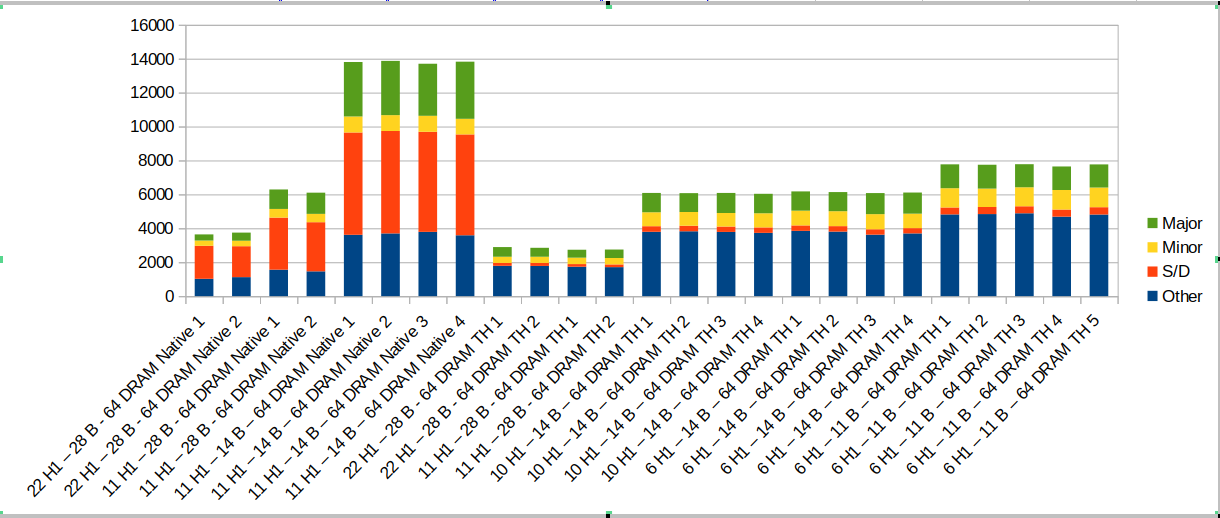
\includegraphics[width=13cm,height=6cm]{lr64.png}
\end{figure*}

\begin{figure*}[h!]
        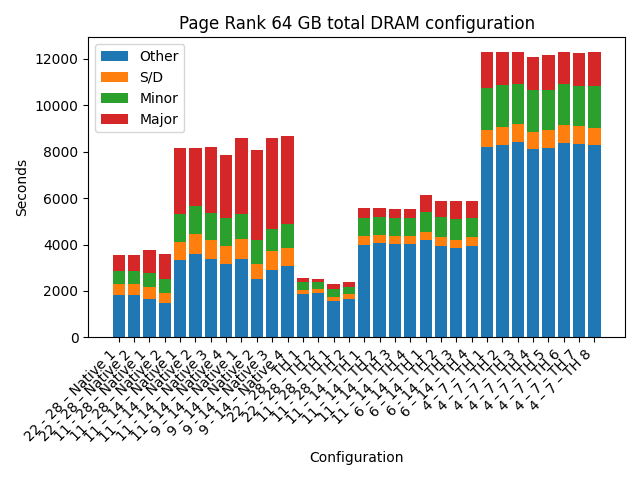
\includegraphics[width=13cm,height=6cm]{pr64.png}
\end{figure*}

\begin{figure*}[h!]
        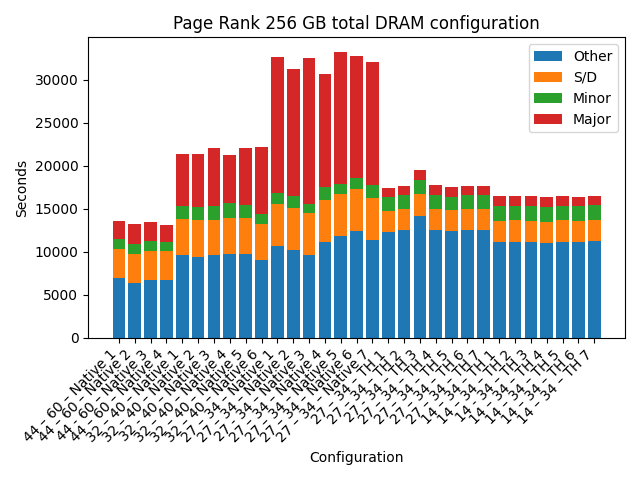
\includegraphics[width=13cm,height=6cm]{pr256.png}
\end{figure*}

\begin{figure*}[h!]
        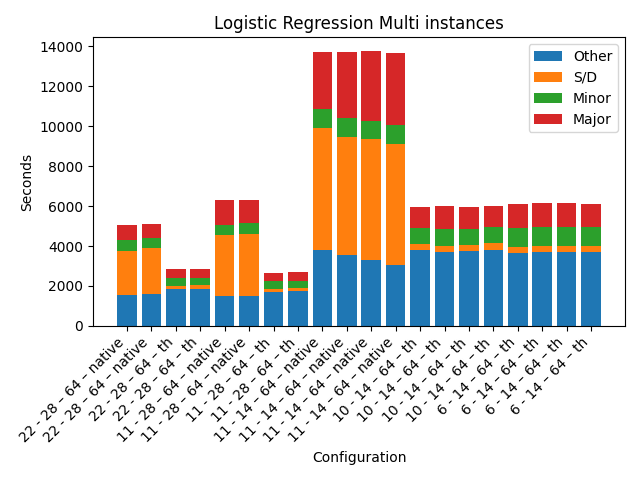
\includegraphics[width=13cm,height=6cm]{logr64.png}
\end{figure*}

\begin{figure*}[h!]
        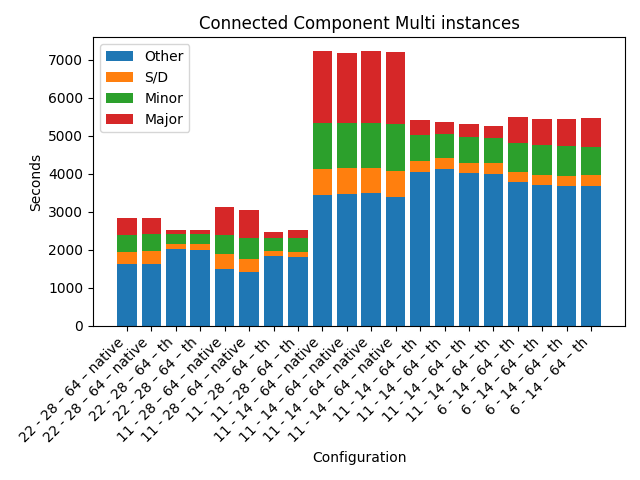
\includegraphics[width=13cm,height=6cm]{cc64.png}
\end{figure*}


\section*{4.1 Are GC and S/D still the main overheads of Native Spark when running multiple spark instances and can TeraHeap increase throughput/number of instances running by reducing these costs? What happens with Java Heap and I/O Cache?}

Figure 18 shows the performance of multiple Native-TeraHeap Spark instances running LinearRegression with 64 GB dataset per instance in our 64 GB DRAM machine. Each instance of Spark uses one executor with 8 cores per executor. Available DRAM is 56 GB and 8 GB are left to the Operating system, resulting in 64 GB total DRAM. Starting from the left of the graph, the first 2 bars show the performance of Native Spark with each instance using 22 GB DRAM for H1 (Java Heap) and 6 GB for JVM Native memory and I/O cache resulting in a total of 28 GB DRAM per instance and utilizing 56 of 64 GB total DRAM. The next 2 bars show the performance of Native Spark with each instance using 11 GB DRAM for H1 (Java Heap) and 17 GB for JVM Native memory and I/O cache resulting in a total of 28 GB DRAM per instance and utilizing 56 of 56 GB total available DRAM. The next 4 bars show the performance of Native Spark with each instance using 11 GB DRAM for H1 (Java Heap) and 3 GB for JVM Native memory and I/O cache resuting in a total of 14 GB DRAM per instance and utilizing 56 of 56 GB total available DRAM. 
The next 2 bars show the performance of TeraHeap Spark with each instance using 22 GB DRAM for H1 (Java Heap) and 6 GB for JVM Native memory and I/O cache resulting in a total of 28 GB DRAM per instance and utilizing 56 of 56 GB total available DRAM. The next 2 bars show the performance of TeraHep Spark with each instance using 11 GB DRAM for H1 (Java Heap) and 17 GB for JVM Native memory and I/O cache resulting in a total of 28 GB DRAM per instance and utilizing 56 of 56 GB total available DRAM. The next 4 bars show the performance of TeraHeap Spark with each instance using 11 GB DRAM for H1 (Java Heap) and 3 GB for JVM Native memory and I/O cache resuting in a total of 14 GB DRAM per instance and utilizing 56 of 56 GB total available DRAM. The next 4 bars show the performance of TeraHeap Spark with increased PageCache and reduced H1 with each instance using 6 GB DRAM for H1 (Java Heap) and 8 GB for JVM Native memory and I/O cache resuting in a total of 14 GB DRAM per instance and utilizing 56 of 56 GB total available DRAM. The next 4 bars show the performance of TeraHeap Spark with increased PageCache and reduced H1 with each instance using 6 GB DRAM for H1 (Java Heap) and 8 GB for JVM Native memory and I/O cache resuting in a total of 14 GB DRAM per instance and utilizing 56 of 56 GB total available DRAM. The last 4 bars show the performance of TeraHeap Spark with increased PageCache and reduced H1 with each instance using 6 GB DRAM for H1 (Java Heap) and 5 GB for JVM Native memory and I/O cache resuting in a total of 14 GB DRAM per instance and utilizing 56 of 56 GB total available DRAM.
By looking at this graph it is clear that Spark suffers by both S/D and GC, but more specifically when it comes to LinerRegression S/D is higher than PageRank. Furthermore we witness Major GC to increase dramaticaly as we increase the number of Spark instances running, same as with PageRank. These overheads are absorbed by TeraHeap. Finally someone would prefer to have a bigger heap than I/O cache when running LinearRegression as well.

Figure 19 shows the performance of multiple Native-TeraHeap Spark instances running PageRank with 8 GB dataset per instance in our 64 GB DRAM machine. Each instance of Spark uses one executor with 8 cores per executor. Available DRAM is 56 GB and 8 GB are left to the Operating system, resulting in 64 GB total DRAM. Starting from the left of the graph, the first 2 bars show the performance of Native Spark with each instance using 22 GB DRAM for H1 (Java Heap) and 6 GB for JVM Native memory and I/O cache resulting in a total of 28 GB DRAM per instance and utilizing 56 of 64 GB total DRAM. The next 2 bars show the performance of Native Spark with each instance using 11 GB DRAM for H1 (Java Heap) and 17 GB for JVM Native memory and I/O cache resulting in a total of 28 GB DRAM per instance and utilizing 56 of 56 GB total available DRAM. The next 4 bars show the performance of Native Spark with each instance using 11 GB DRAM for H1 (Java Heap) and 3 GB for JVM Native memory and I/O cache resuting in a total of 14 GB DRAM per instance and utilizing 56 of 56 GB total available DRAM. The next 4 bars show the performance of TeraHeap Spark with increased PageCache and reduced H1 with each instance using 9 GB DRAM for H1 (Java Heap) and 5 GB for JVM Native memory and I/O cache resuting in a total of 14 GB DRAM per instance and utilizing 56 of 56 GB total available DRAM. 
The next 2 bars show the performance of TeraHeap Spark with each instance using 22 GB DRAM for H1 (Java Heap) and 6 GB for JVM Native memory and I/O cache resulting in a total of 28 GB DRAM per instance and utilizing 56 of 56 GB total available DRAM. The next 2 bars show the performance of TeraHep Spark with each instance using 11 GB DRAM for H1 (Java Heap) and 17 GB for JVM Native memory and I/O cache resulting in a total of 28 GB DRAM per instance and utilizing 56 of 56 GB total available DRAM. The next 4 bars show the performance of TeraHeap Spark with each instance using 11 GB DRAM for H1 (Java Heap) and 3 GB for JVM Native memory and I/O cache resuting in a total of 14 GB DRAM per instance and utilizing 56 of 56 GB total available DRAM. The next 4 bars show the performance of TeraHeap Spark with increased PageCache and reduced H1 with each instance using 6 GB DRAM for H1 (Java Heap) and 8 GB for JVM Native memory and I/O cache resuting in a total of 14 GB DRAM per instance and utilizing 56 of 56 GB total available DRAM. The last 8 bars show the performance of TeraHeap Spark with each instance using 4 GB DRAM for H1 (Java Heap) and 3 GB for JVM Native memory and I/O cache resuting in a total of 7 GB DRAM per instance and utilizing 56 of 56 GB total available DRAM.  
By looking at this graph it is clear that Spark suffers by both S/D and GC, but more specifically when it comes to PageRank we witness Major GC to increase dramaticaly as we increase the number of Spark instances running. These overheads are absorbed by TeraHeap. TeraHeap also scales to 8 instances while Native can't because it runs out of memory. Finally someone would prefer to have a bigger heap than I/O cache when running PageRank.

Figure 20 shows the performance of multiple Native-TeraHeap Spark instances running PageRank with 32 GB dataset per instance in our 256 GB DRAM machine. Each instance of Spark uses one executor with 8 cores per executor. Available DRAM is 240 GB and 16 GB are left to the Operating system, resulting in 256 GB total DRAM. Starting from the left of the graph, the first 4 bars show the performance of Native Spark with each instance using 44 GB DRAM for H1 (Java Heap) and 16 GB for JVM Native memory and I/O cache resulting in a total of 60 GB DRAM per instance and utilizing 240 of 256 GB total DRAM. The next 6 bars show the performance of Native Spark with each instance using 32 GB DRAM for H1 (Java Heap) and 8 GB for JVM Native memory and I/O cache resulting in a total of 40 GB DRAM per instance and utilizing 240 of 240 GB total available DRAM. The next 7 bars show the performance of Native Spark with each instance using 27 GB DRAM for H1 (Java Heap) and 7 GB for JVM Native memory and I/O cache resuting in a total of 34 GB DRAM per instance and utilizing 240 of 240 GB total available DRAM. The next 7 bars show the performance of TeraHeap Spark with each instance using 27 GB DRAM for H1 (Java Heap) and 7 GB for JVM Native memory and I/O cache resuting in a total of 34 GB DRAM per instance and utilizing 240 of 240 GB total available DRAM. The last 7 bars show the performance of Native Spark with each instance using 14 GB DRAM for H1 (Java Heap) and 20 GB for JVM Native memory and I/O cache resuting in a total of 34 GB DRAM per instance and utilizing 240 of 240 total DRAM. By looking at this graph it is clear that Spark suffers by both S/D and GC, but more specifically when it comes to PageRank we witness Major GC to increase dramaticaly as we increase the number of Spark instances running. These overheads are absorbed by TeraHeap.
Finally someone would prefer to have a bigger heap than I/O cache when running PageRank.

\begin{figure*}[h!]
        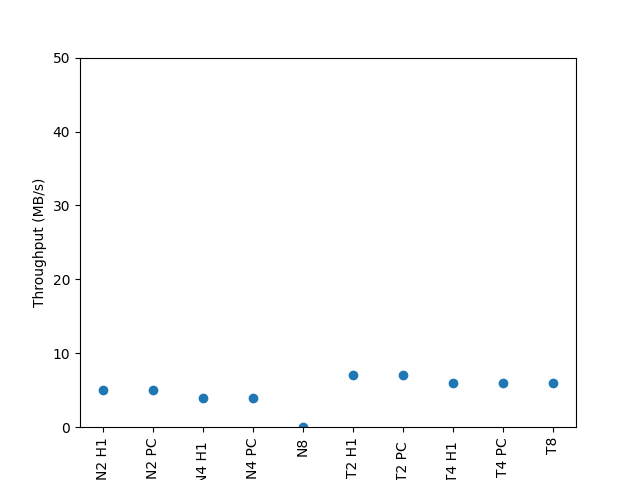
\includegraphics[width=13cm,height=6cm]{PR_64_THR.png}
\end{figure*}

\begin{figure*}[h!]
        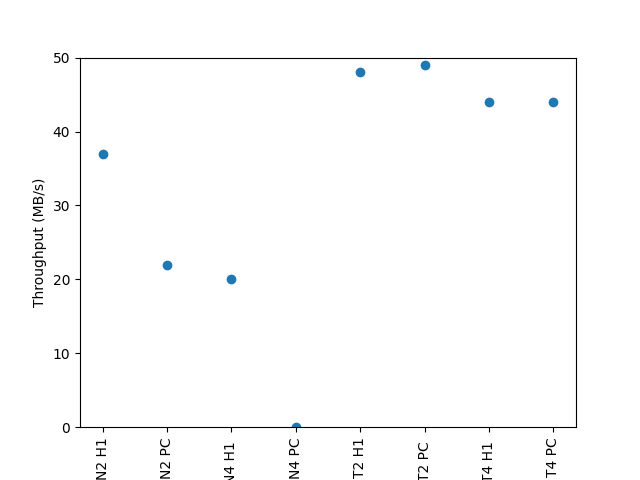
\includegraphics[width=13cm,height=6cm]{LINR_64_THR.png}
\end{figure*}

\begin{figure*}[h!]
        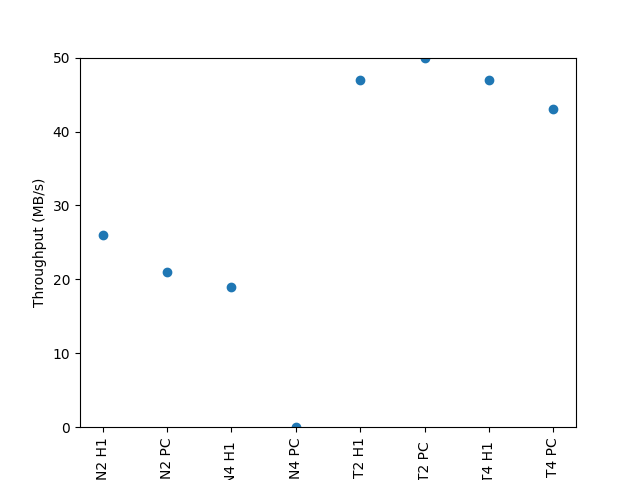
\includegraphics[width=13cm,height=6cm]{LOGR_64_THR.png}
\end{figure*}

\begin{figure*}[h!]
        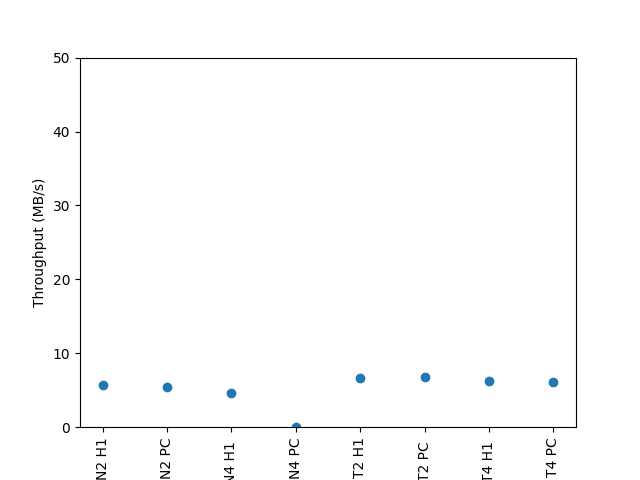
\includegraphics[width=13cm,height=6cm]{CC_64_THR.png}
\end{figure*}

\begin{figure*}[h!]
        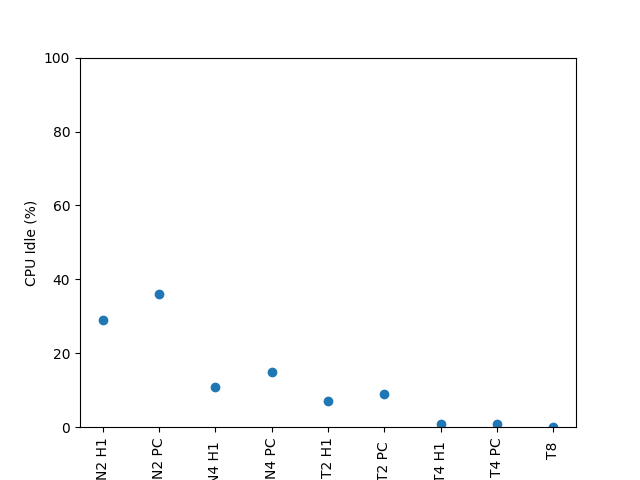
\includegraphics[width=13cm,height=6cm]{PR_64_IDLE.png}
\end{figure*}

\begin{figure*}[h!]
        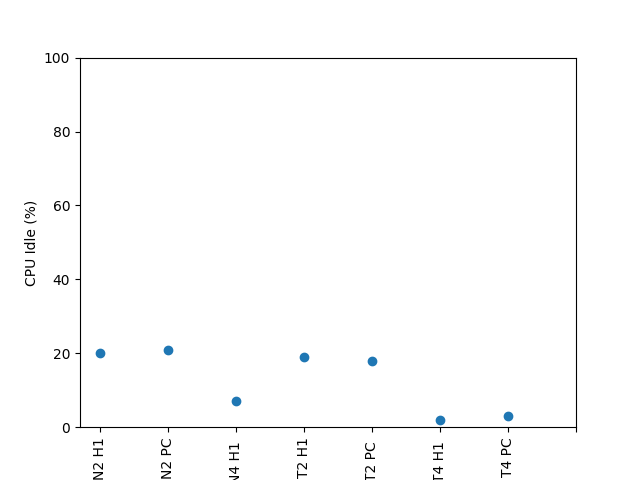
\includegraphics[width=13cm,height=6cm]{LINR_64.png}
\end{figure*}

\begin{figure*}[h!]
        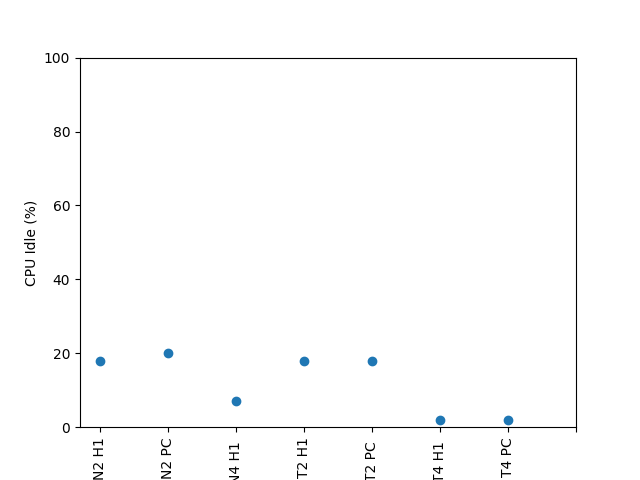
\includegraphics[width=13cm,height=6cm]{LOGR_64.png}
\end{figure*}

\begin{figure*}[h!]
        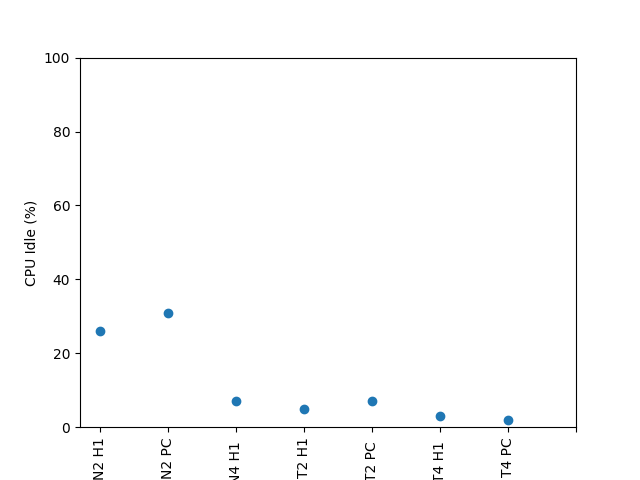
\includegraphics[width=13cm,height=6cm]{CC_64.png}
\end{figure*}

By looking at figures 21-23 we see that Native Spark's throughput decreases as the number of colocated instances-executors increase in the server. The main goal for colocating tasks is to increase the CPU utilization and achieve better throughput as fast as possible as if running each instance isolated. While Native Spark fails to provide scalability, TH Spark achieves nearly double the throughput of Native Spark and is also able to scale beyond 4 instances as we see in figures 24-26.

Figures 27-29 show the percentage of idle CPU while the number of colocated instances grows. CPU idle should decrease in this particular concept and that is something proven in the figure. In PageRank graph we notice TeraHeap with 2 instances achieving less idle CPU percentage than Native Spark with 4 instances.
\begin{figure*}[h!]
        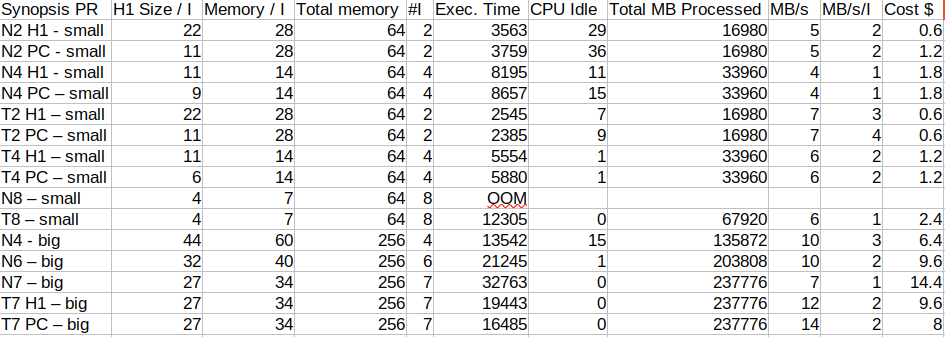
\includegraphics[width=18cm,height=5cm]{pr_table.png}
\end{figure*}

\begin{figure*}[h!]
        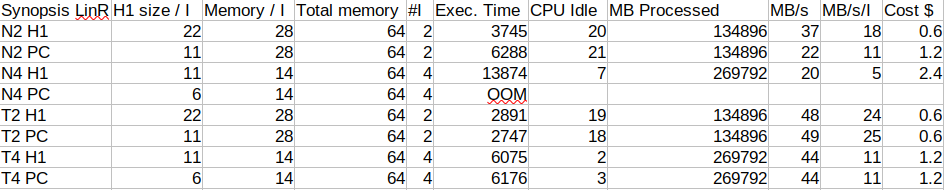
\includegraphics[width=20cm,height=10cm]{linr_table.png}
\end{figure*}

\begin{figure*}[h!]
        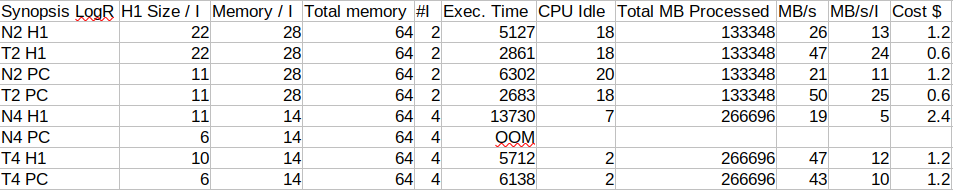
\includegraphics[width=20cm,height=10cm]{logr_table.png}
\end{figure*}

\begin{figure*}[h!]
        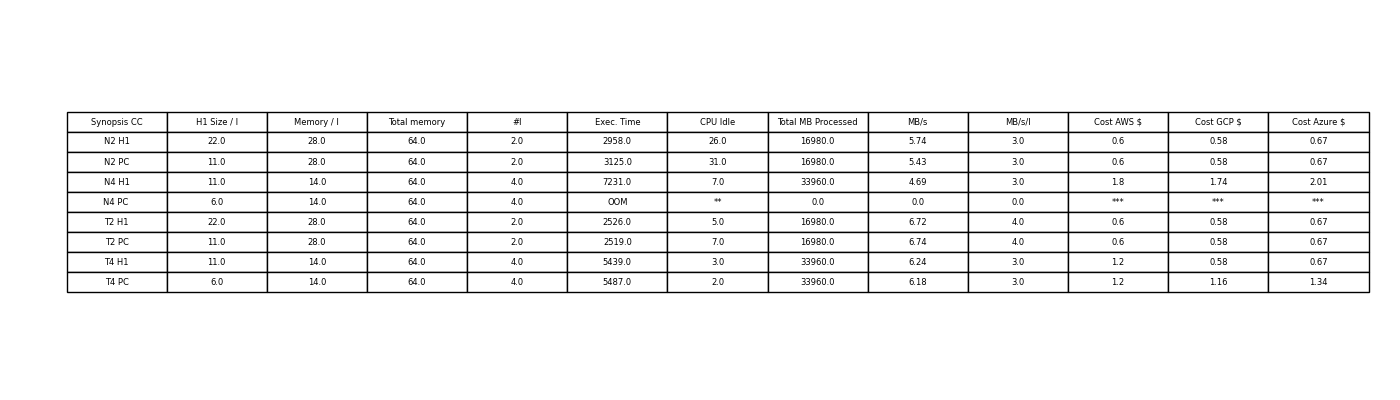
\includegraphics[width=20cm,height=10cm]{cc_table.png}
\end{figure*}


Tables 1, 2 and 3 show a detailed synopsis of the performance and AWS cost of deploying multiple instances of Spark using both techniques. Each setup is run using 2 different amounts for H1 (80 and 40\%). While the number of instances increases TeraHeap appears to maintain throughput while Native Spark has significant throughput decrease. In several occassions, if we compare Native's to TeraHeap's throughput we notice TeraHeap having more than 100\% increase compared to Native. In PageRank's 64 DB DRAM setup TeraHeap manages to scale to 8 instances while Native Spark runs out of memory. Furthermore when looking at the PageRank table it becomes clear that TeraHeap achieves a higher CPU utilization, because of the S/D elimination and less I/O. 

%%%%%%%%%%%%%%%%%%%%%%%%%%%%%%%%%%%%%%%%%%%%%%%%%%%%%%%%%%%%%%%%%%%%%%
\section*{5. Future Work}

While our proposed offloading technique shows promising results in improving job throughput for big data analytics workloads on Spark clusters, there are several avenues for future work to further improve the performance and scalability of Spark clusters. 

Firstly, one potential direction for future work is to investigate the use of other types of storage mediums such as the hybrid NVM. This medium could improve the performance of Big data analytics further by combining the advantages of memory and storage.

Secondly, another area for future work is to develop techniques for dynamically adjusting the heap offloading decisions based on workload characteristics and resource availability. For example, the offloading decision can be based on the size of the input data or the availability of DRAM capacity in the cluster. Such techniques can help maximize the performance gains achieved by offloading while minimizing the cost of offloading.

Thirdly, an interesting direction for future work is to explore the use of heap offloading in environments where Spark clusters are deployed across multiple machines using RDMA to achieve communication between the different machines. This can help utilize the DRAM, CPU and storage availability in more than one machine and provide a more cost-effective solution for big data processing.

Finally, another potential area for future work is to investigate the use of heap offloading for other big data processing frameworks beyond Spark. Many other big data processing frameworks such as Apache Giraph can potentially benefit from offloading techniques to improve their performance and scalability.

Overall, there are many exciting avenues for future work in improving the performance and scalability of big data processing frameworks such as Spark. Our proposed offloading technique provides a solid foundation for future work and offers a promising approach for addressing the challenges of big data processing.

%%%%%%%%%%%%%%%%%%%%%%%%%%%%%%%%%%%%%%%%%%%%%%%%%%%%%%%%%%%%%%%%%%%%%%
\section*{6. Conclusion}

In this paper, we proposed a new technique for improving the performance and job throughput of Spark clusters by moving parts of the managed Java Heap to a secondary memory-mapped heap over fast storage devices such as NVMe. Our approach leverages the capabilities of the underlying running machine to free computation-intensive tasks running on the Spark workers from memory pressure, thereby reducing the workload on the workers and improving their performance and job throughput.

Our experimental results demonstrate the effectiveness of our approach using various big data analytics workloads on a Spark cluster. We also compare our approach with the native Spark distribution and showed that our approach can be used instead of this distribution to further improve performance.

Our work contributes to the growing body of research on improving the performance and scalability of Spark clusters for big data analytics workloads. Our approach offers a scalable solution for processing increasingly large and complex big data workloads and can be easily integrated into existing Spark clusters.

Overall, our offloading technique offers a promising approach to improving job throughput for big data analytics workloads on Spark clusters, particularly for computation-intensive tasks. With the increasing demand for efficient and scalable big data processing frameworks, our approach provides a valuable contribution to the field of big data analytics and memory management.

% Here's where you specify the bibliography style file.
% The full file name for the bibliography style file 
% used for an ASME paper is asmems4.bst.
\bibliographystyle{asmems4}


%%%%%%%%%%%%%%%%%%%%%%%%%%%%%%%%%%%%%%%%%%%%%%%%%%%%%%%%%%%%%%%%%%%%%%
\begin{acknowledgment}
	Still an empty section.
\end{acknowledgment}

%%%%%%%%%%%%%%%%%%%%%%%%%%%%%%%%%%%%%%%%%%%%%%%%%%%%%%%%%%%%%%%%%%%%%%
% The bibliography is stored in an external database file
% in the BibTeX format (file_name.bib).  The bibliography is
% created by the following command and it will appear in this
% position in the document. You may, of course, create your
% own bibliography by using thebibliography environment as in
%
% \begin{thebibliography}{12}
% ...
% \bibitem{itemreference} D. E. Knudsen.
% {\em 1966 World Bnus Almanac.}
% {Permafrost Press, Novosibirsk.}
% ...
% \end{thebibliography}

% Here's where you specify the bibliography database file.
% The full file name of the bibliography database for this
% article is asme2e.bib. The name for your database is up
% to you.
\bibliography{asme2e}

\nocite{*}

\end{document}
